\documentclass{article}

%%% Fill details here (in the second brackets)
\newcommand{\name}{Sam Teeter}     % Your name (First Last)
\newcommand{\wustlkey}{teeters}             % Your WUSTL Key
%%%



%%%%%%%%%%%%%%%%%%%%%% Formatting Stuff %%%%%%%%%%%%%%%%%%%%%%%%%%%
\usepackage{times}
\usepackage[T1]{fontenc}

\setlength{\parskip}{1em}\setlength{\parindent}{0pt}
\linespread{1.25}
\usepackage[margin=0.7in,top=1in]{geometry}\usepackage{fancyhdr}
\pagestyle{fancy}\lhead{\bf \name}\rhead{\bf \wustlkey}\cfoot{\thepage}
\newcommand{\info}{\clearpage \subsection*{Information}}
\newcommand{\solution}[1]{\clearpage \subsection*{Solution #1}}
\newcommand{\spart}[1]{\paragraph{(#1)}}
%%%%%%%%%%%%%%%%%%%%%%%%%%%%%%%%%%%%%%%%%%%%%%%%%%%%%%%%%%%%%%%%%%%


%%% Add any more packages if you want to
\usepackage{amsmath,graphicx}


\begin{document}
%%%%% Main Body goes here

% Begin solution to every problem like this.
\solution{1}

\spart{a} Because $(x-y)^2 + \lambda|x|$ is discontinuous at $x=0$, we can minimize it by finding the minima over the piecewise regions $(-\infty, 0)$ and $(0, \infty)$. Differentiating the expression with respect to $x$, we have
\begin{equation}
2(x-y) + \lambda \text{sign}(x) = 0
\end{equation}
which resolves to 
\begin{equation}
x = y - \frac{1}{2} \text{sign}(x) \lambda
\end{equation}

Note that if we plug this back into the original expression, we get
\begin{equation}
\text{cost} = \frac{1}{4} \lambda^2+\lambda|x|
\end{equation}
If we assume that $\lambda>0$, this expression is minimized by the $x$ with the smallest absolute value. In this case we can write
\begin{equation}
x = y-\frac{1}{2} \text{sign}(y)\lambda
\end{equation}

\spart{b} Here is the denoised image using the default initial value of $\lambda$, 0.88. I found that lower values of $\lambda$ resulted in an image more similar to the input, whereas higher values of $\lambda$ resulted in images closer to a uniform gray. 

\begin{figure*}[!h]
\centering
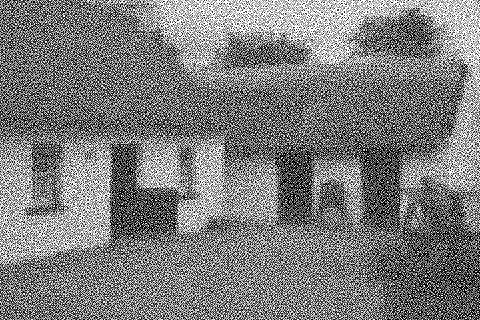
\includegraphics[width=0.5\textwidth]{code/outputs/prob1.png}
\caption{Denoised output}
\end{figure*}

\solution{2}

\spart{a} White-balanced outputs:

\begin{figure*}[!h]
  \centering
  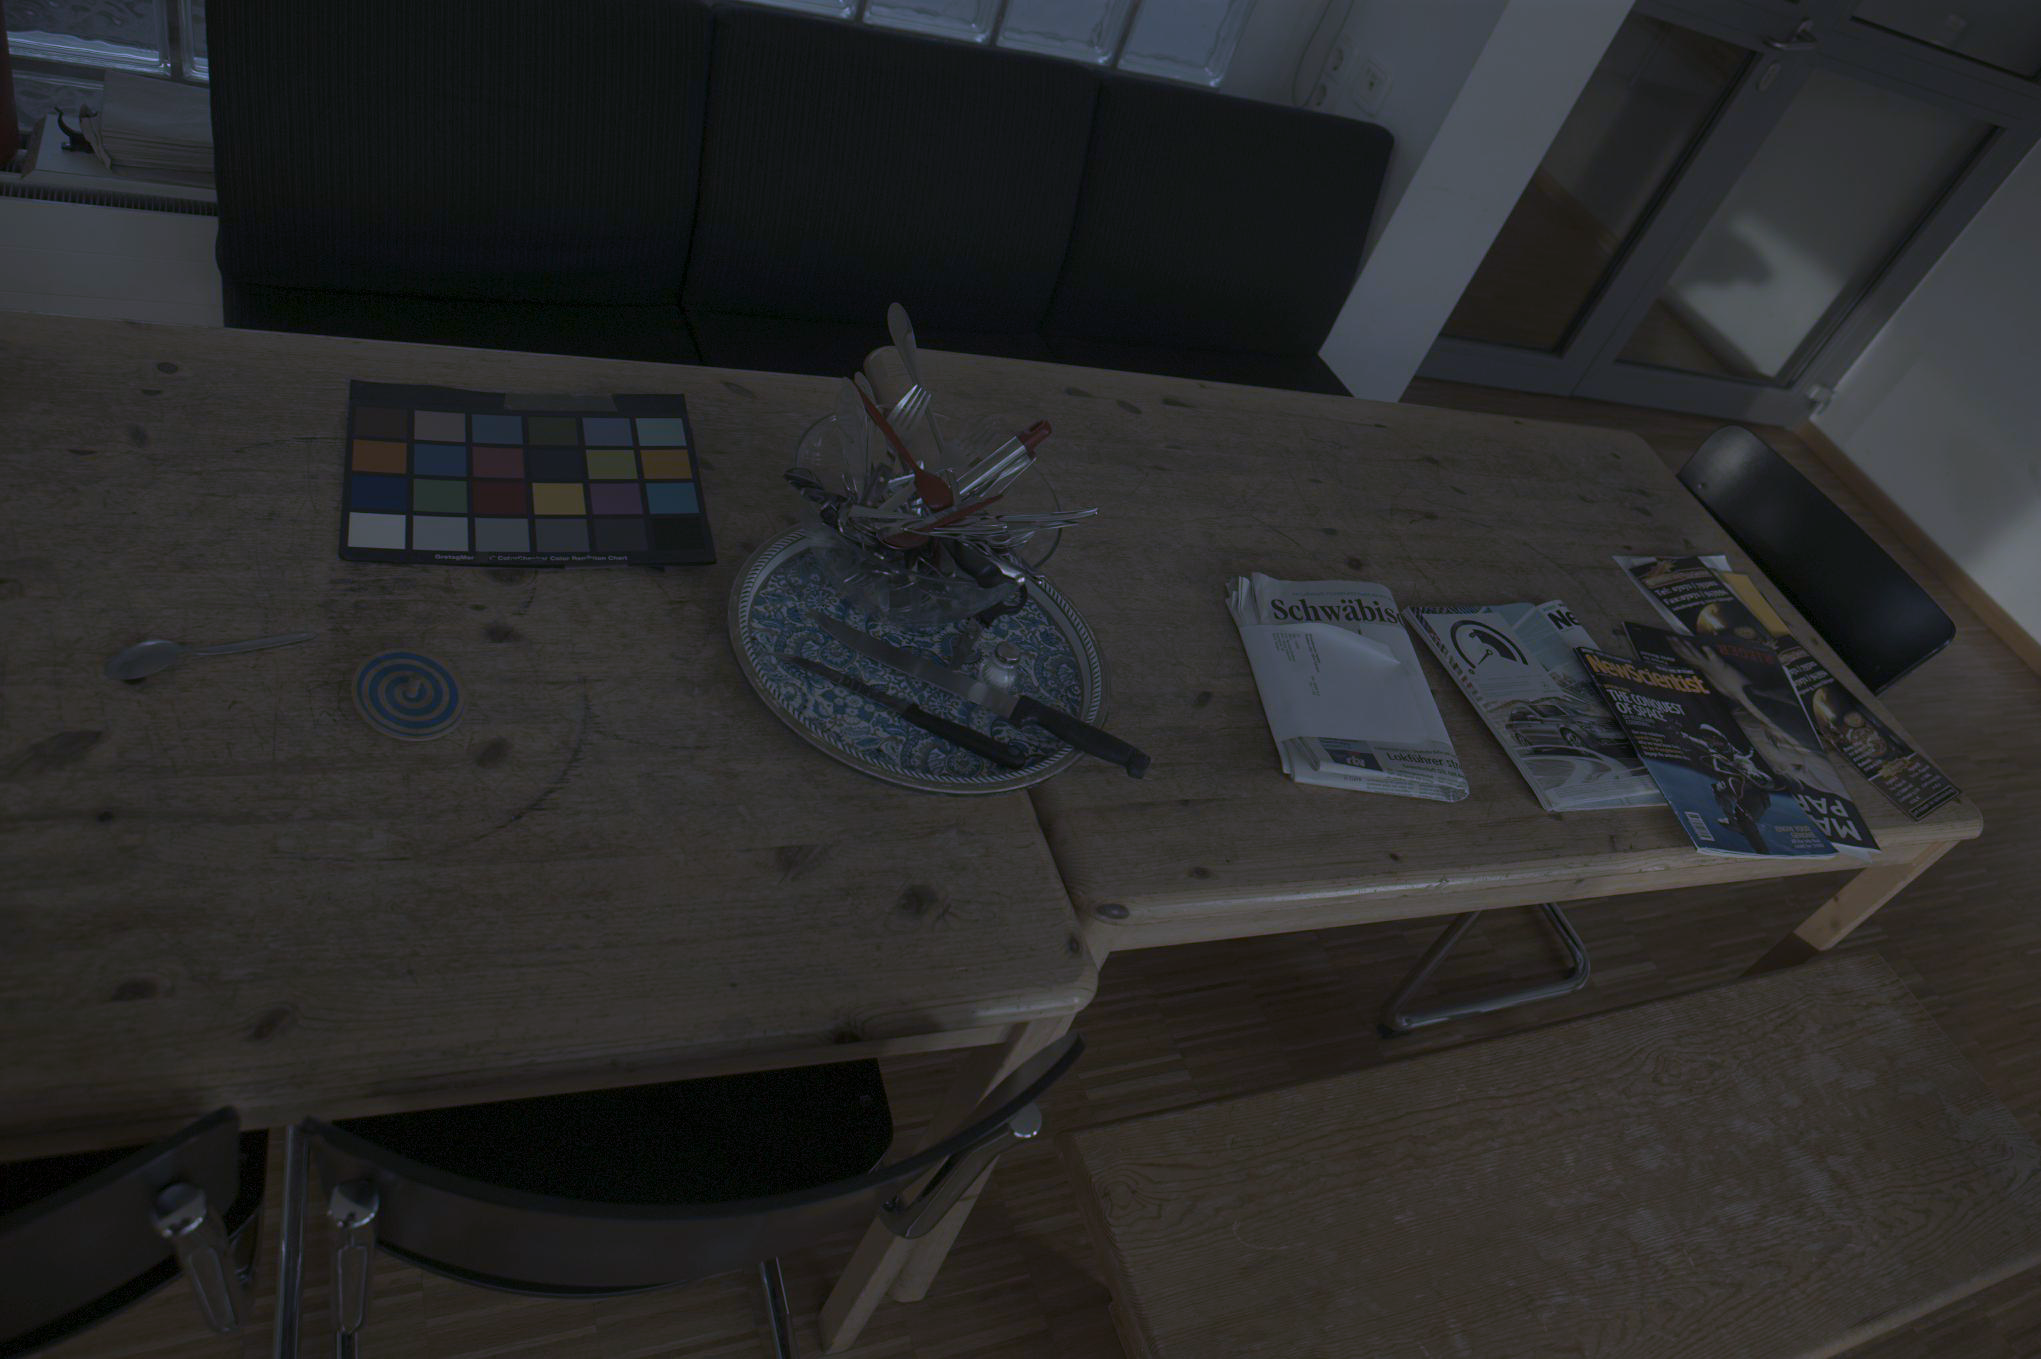
\includegraphics[height=10em]{code/outputs/prob2a_1.png}
  \caption{Image 1}
\end{figure*}

\begin{figure*}[!h]
  \centering
  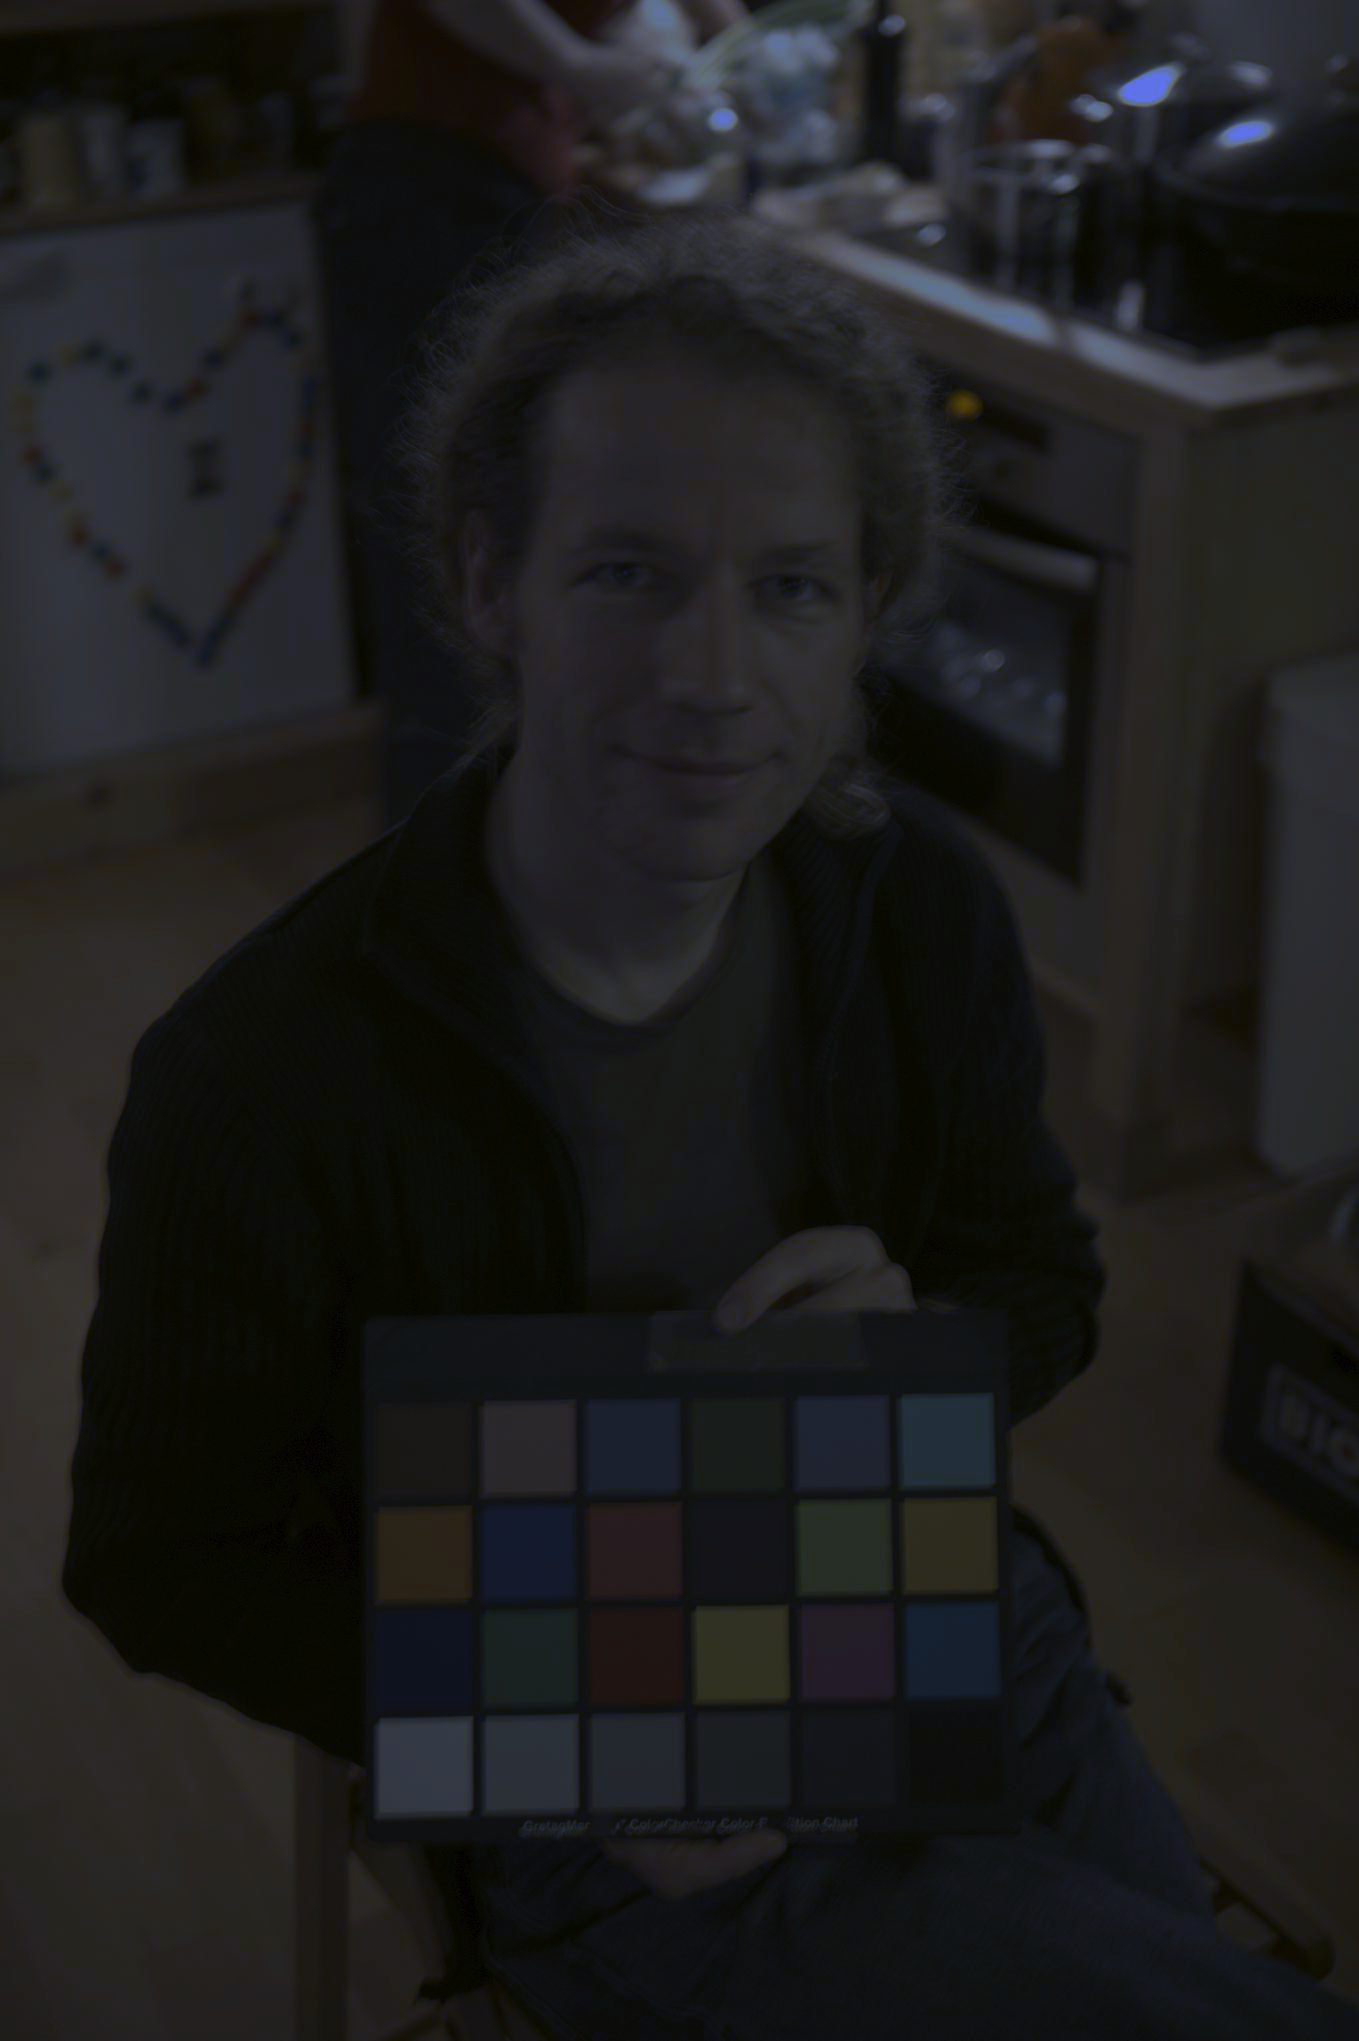
\includegraphics[height=10em]{code/outputs/prob2a_2.png}
  \caption{Image 2}
\end{figure*}

\begin{figure*}[!h]
  \centering
  \includegraphics[height=10em]{code/outputs/prob2a_3.png}
  \caption{Image 3}
\end{figure*}

\spart{b} White-balanced outputs using the top 10\% of color intensities:

\begin{figure*}[!h]
  \centering
  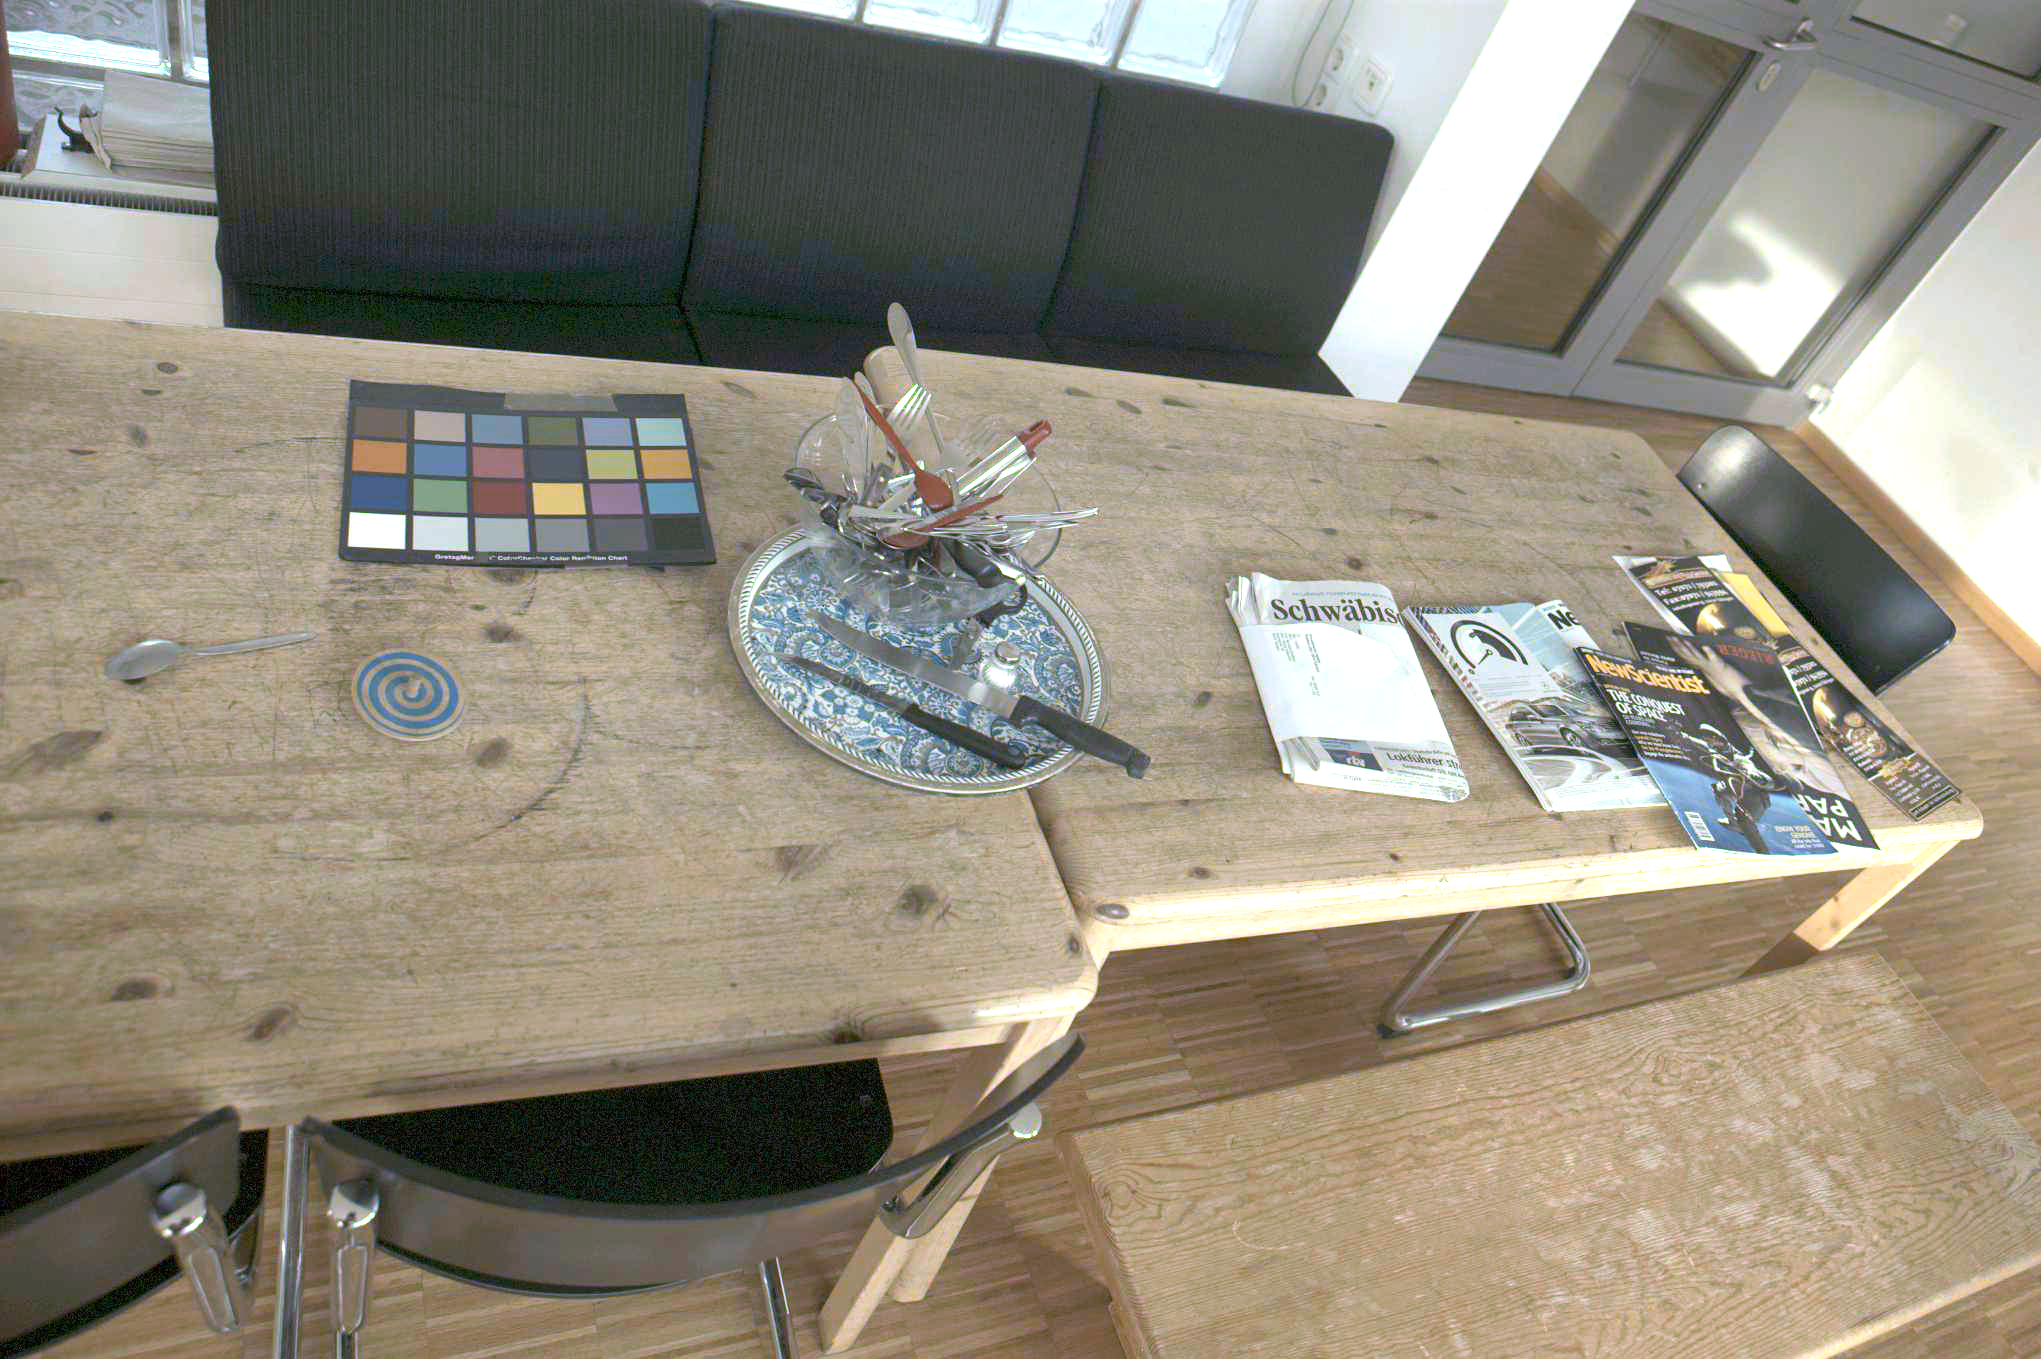
\includegraphics[height=10em]{code/outputs/prob2b_1.png}
  \caption{Image 1}
\end{figure*}

\begin{figure*}[!h]
  \centering
  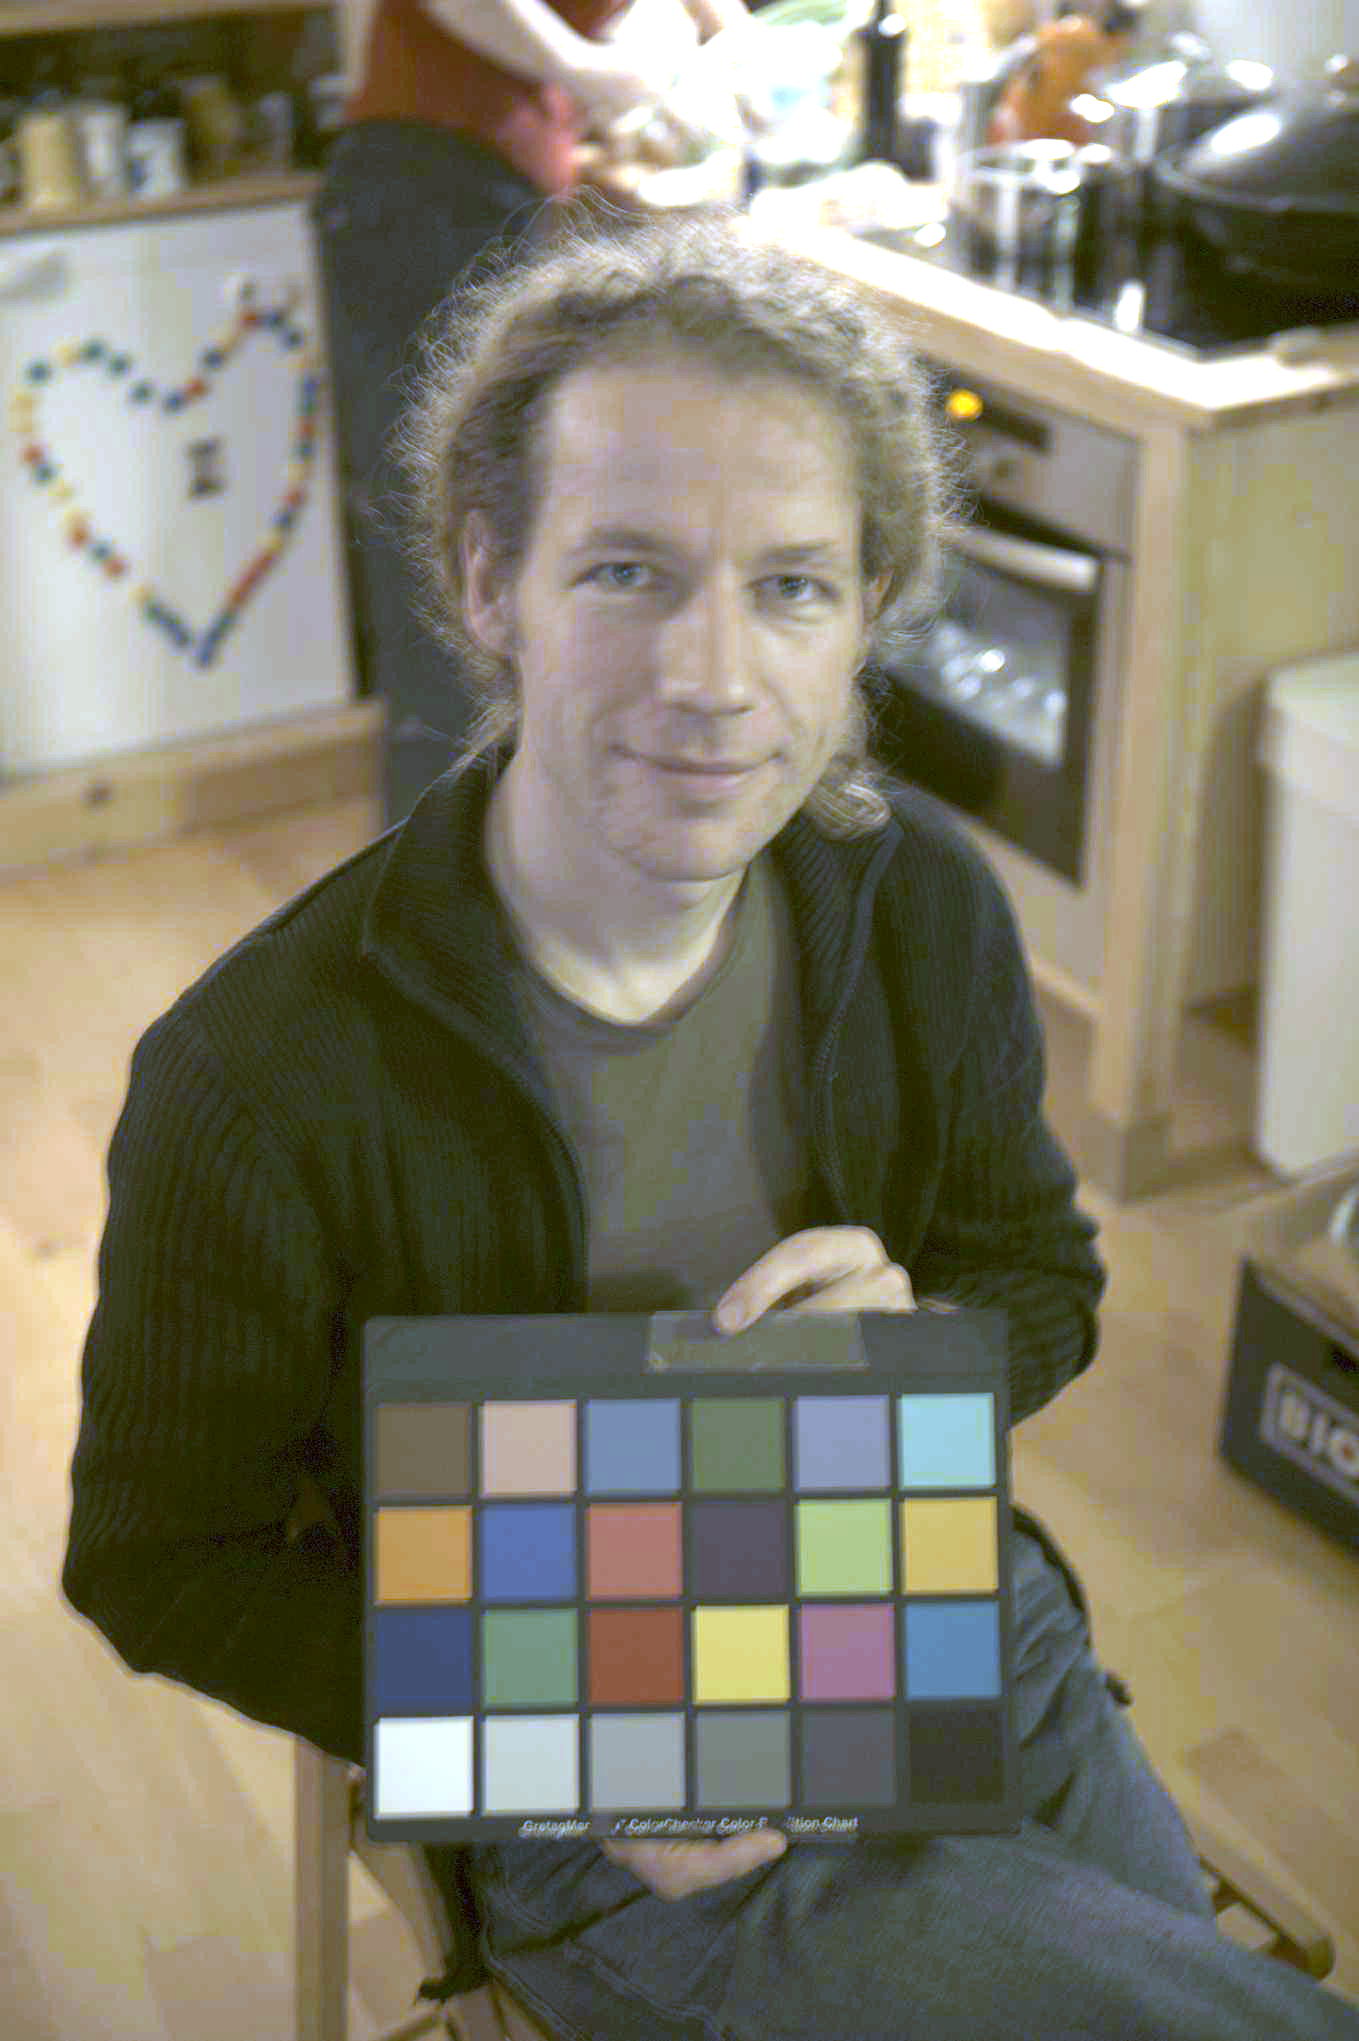
\includegraphics[height=10em]{code/outputs/prob2b_2.png}
  \caption{Image 2}
\end{figure*}

\begin{figure*}[!h]
  \centering
  \includegraphics[height=10em]{code/outputs/prob2b_3.png}
  \caption{Image 3}
\end{figure*}


\solution{3} 

\spart{a}

\begin{figure*}[!h]
  \centering
  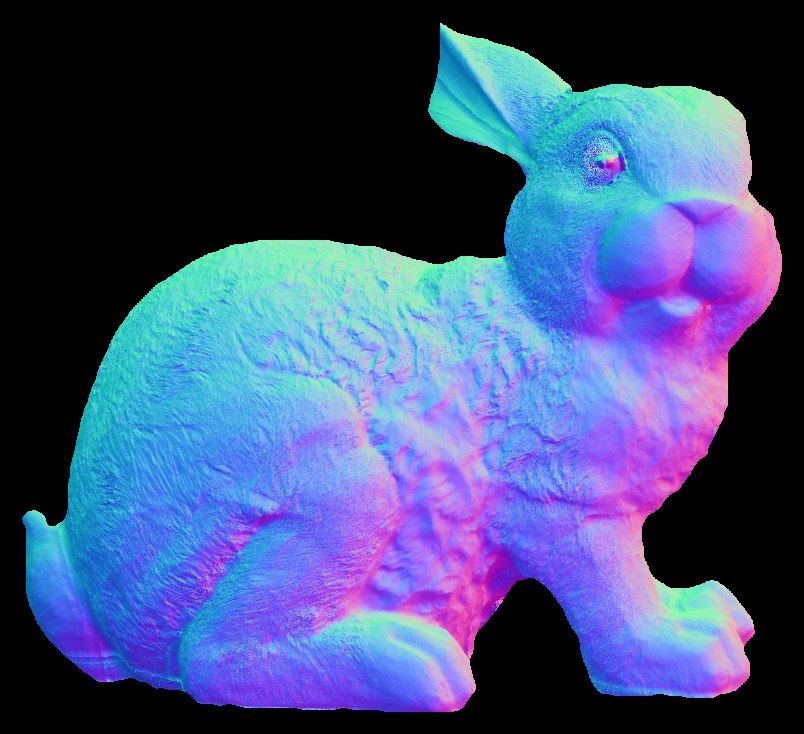
\includegraphics[height=20em]{code/outputs/prob3_nrm.png}
  \caption{Surface normals}
\end{figure*}

\spart{b}

\begin{figure*}[!h]
  \centering
  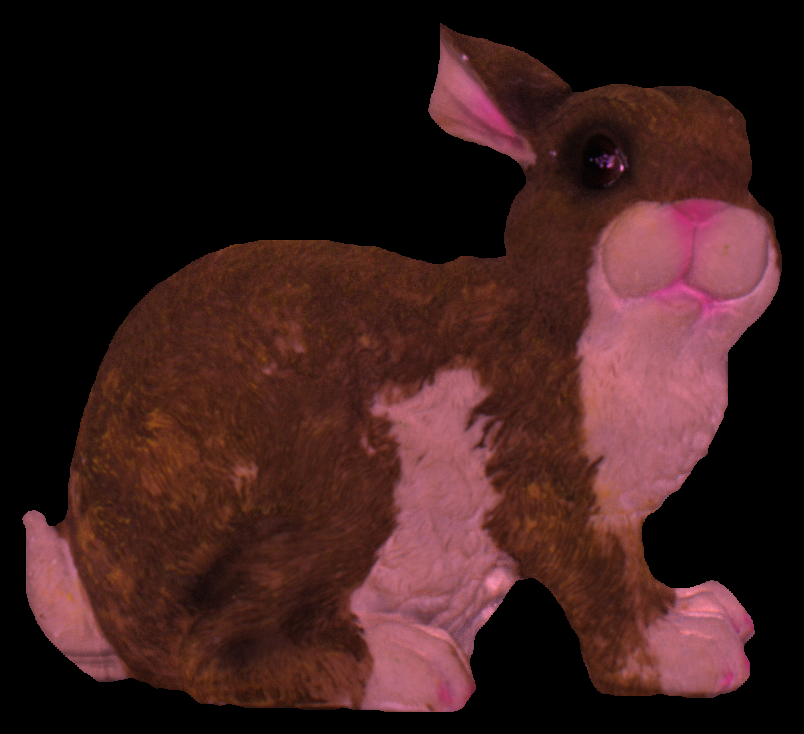
\includegraphics[height=20em]{code/outputs/prob3_alb.png}
  \caption{Albedo}
\end{figure*}

\solution{4}

\begin{figure*}[!h]
  \centering
  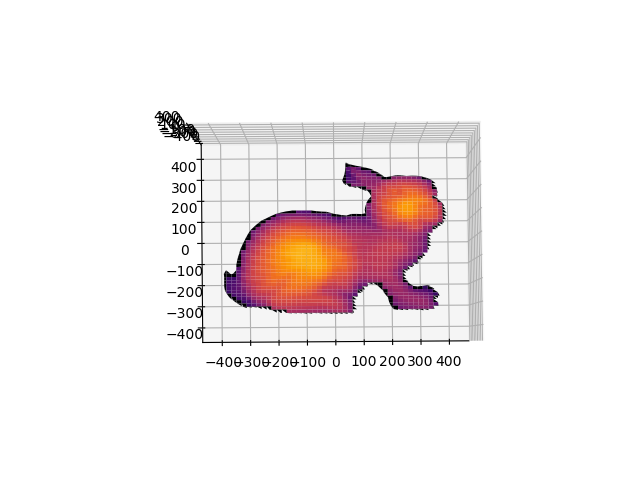
\includegraphics[height=20em]{prob4.png}
  \caption{Depth map using Fourier transforms}
\end{figure*}

\solution{5}

Side note: I was curious about the magnitude of the gradient over time, so I had my program output the magnitude of the change in $Z$ for each iteration (measured by the Euclidean norm). After 200 iterations, it dropped to about 80, and the change in the depth map was not as noticeable.

\begin{figure*}[!h]
  \centering
  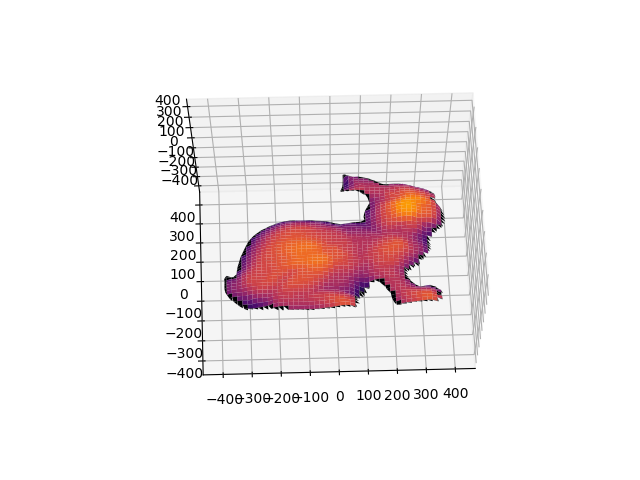
\includegraphics[height=20em]{prob5.png}
  \caption{Depth map after 200 iterations}
\end{figure*}


\info

This problem set took approximately 16 hours of effort.


I discussed this problem set with:
\begin{itemize}
\item Jarrett Gross
\end{itemize}


% Note that you might have to escape some special symbols in URLS like \_
I also got hints from the following sources:
\begin{itemize}
\item Numpy documentation
\end{itemize}

\end{document}
